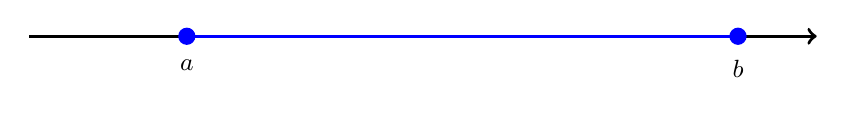
\begin{tikzpicture}
  \def\a{-3}
  \def\b{4}
  
  \coordinate (A) at (-5,0);
  \coordinate (B) at (5,0);

  \coordinate (P) at (\a,0);
  \coordinate (Q) at (\b,0);
  
  \draw [very thick,\lt->] (A) -- (B);
  \draw [very thick,blue] (P) -- (Q);

  \draw [very thick,blue,fill=blue] (P) circle (2.5pt);
  \draw [very thick,blue,fill=blue] (Q) circle (2.5pt);
   
  %% \draw [very thick] (\a,2.5pt) -- +(0,-5pt) node [anchor=north, font=\small] {$a$};
  %% \draw [very thick] (\b,2.5pt) -- +(0,-5pt) node [anchor=north, font=\small] {$b$};

  \node [anchor=north, font=\small] at (\a,-5pt) {$a$};
  \node [anchor=north, font=\small] at (\b,-5pt) {$b$};
  
\end{tikzpicture}
